\chapter{Integrating the Law and Software}

Social constraints implied by the law are often overlooked by software
engineers. While many software engineers are justly unconcerned with tortious
product liabilities, those that develop safety-critical applications should be
especially aware of these \textit{integration points}. An integration point, in
the context of this research, is the location of the process area of one system
where another system incorporates itself.

\section{Legal Influence on Software Engineering}

In Figure \ref{fig:LawOnTech} a slice of the software evolution model (Figure
\ref{fig:technical}) is shown in gray. The legal archives from the common law
model of Figure \ref{fig:commonlaw} is shown in white. The integration point
where the law influences software engineering happens during client preparations
and design planning. The bold arrows show where these two models are integrated
together from the legal side to the technical side.

In safety-critical systems, legal data should be utilized during these phases of
the software lifecycle. Instead of making these plans in isolation, software
engineers should design safety into their products using the considerations laid
out by the law. There are several ways that the legal archives present
themselves to software designers.

\begin{figure}[t]
\begin{center}
\includegraphics{figures/LawOnTech.eps}
\end{center}
\caption{Law Influences Technical Innovation}
\label{fig:LawOnTech}
\end{figure}

\subsection{Statutory Law}
\subsection{Common Law Precedent}

\section{Software Engineering Influence on Legal Rules}

Software engineers have a voice as to what gets decided in legal disputes.

\subsection{Expert Testimony}

Oftentimes, legal counsel will try to prove or defend against negligence using
the testimony of an expert in the field. This is often the case in professional
negligence or malpractice disputes. While this has not occurred in software, the
medical field is familiar with this process \cite{Deitschel02}.

\begin{figure}[t]
\begin{center}
\includegraphics{figures/TechOnLaw.eps}
\end{center}
\caption{Technical Innovation Influences Law}
\label{fig:TechOnLaw}
\end{figure}

\subsection{Standards and Committees}
Despite the evidence of ineffective safety assurance \cite{Therac25,Maisel05},
current standards in the software industry illustrate that efforts are being
made to ensure the safety of mission critical software applications. Though
unapproved and unofficial to any governing body, the Software Engineering Code
of Ethics supports these efforts towards safer software. The first principle of
the code requires that software engineers work consistently with the public
interest\footnote{The preamble, the entire listing of ``Principle 1: PUBLIC'',
and the short version of the remaining principles of the Software Engineering
Code of Ethics and Professional Practice are listed in Appendix \ref{A:SECode}}.

This code of ethics is approved by both the IEEE and the ACM. In addition, these
and other professional organizaitons  have developed standards and guidelines
for developers to improve software processes.


\subsection{Education Accreditation}

In the past, ACM and other computer societies have recieved inquiries from
parents, government agencies, and companies that wish to find quality computing
programs \cite{Mulder84}. In response to the educational deficiencies found in
some engineering schools, organizations like the ACM, the Computer Society, and
the Accreditation Board for Engineering and Technology (ABET) formed standards
to evaluate academic programs and accredit schools that meet these standards
\cite{ABET,Mulder84}.

As opposed to science, accreditation is important for engineering because
engineers often deal directly with customers that are neither engineers or
scientists, so a stricter level of care is necessary. Accrediation raises the
quality of education by ensuring that graduates are exposed to the most
important ideas of the field and how to use them \cite{Parnas98}.

\section{Case Study: Evaluating Integration Points}

\subsection{Paving the Intersection}
\singlespace
\begin{longtable}{| p{2in} | p{2in} | p{2in} |}
\caption{Activities, Constraints, and Standards}\label{thetable}\\

\hline
\textbf{Verification Activity} & \textbf{Social Constraints} & \textbf{Standard or Practice}\\
\hline
\endhead

\hline \multicolumn{3}{r}{{Continued on next page}} \\ \hline
\endfoot

\hline \hline
\endlastfoot

\multicolumn{3}{|c|}{\textit{\textbf{1. Requirements}}}\\
\hline
a. Determine verification approach & \multirow{2}{2in}{Insure that the product is reasonably fit
for its intended purposes} & \underline{IEEE Std 1012-2004}:
\begin{small}\begin{itemize}
\item System test plan generation - 5.4.2(5)
\item Acceptance test plan generation - 5.4.2(6)
\end{itemize}\end{small}\\
\cline{1-1} \cline{3-3}
b. Determine adequacy of requirements & & \underline{IEEE Std 1012-2004}:
\begin{small}\begin{itemize}
\item Software requirements evaluation - 5.4.2(2)
\end{itemize}\end{small}\\
\hline
c. Generate functional test data & Tests and inspections match the severity of
the product's expected use & \underline{IEEE Std 1012-2004}:
\begin{small}\begin{itemize}
\item Criticality analysis - 5.4.3(4)
\item Component test plan generation - 5.4.3(5)
\item Integration test plan generation - 5.4.3(6)
\item Component test design generation - 5.4.3(7)
\item Integration test design generation - 5.4.3(8)
\item System test design generation - 5.4.3(9)
\item Acceptance test design generation - 5.4.3(10)
\end{itemize}\end{small}\\
\hline \newpage
\multicolumn{3}{|c|}{\textit{\textbf{2. Design}}}\\
\hline
a. Determine consistency of design with requirements & Insure that the product
is reasonably fit for its intended purposes & \underline{IEEE Std 1012-2004}:
\begin{small}\begin{itemize}
\item Traceability analysis - 5.4.3(1)
\item Software design evaluation - 5.4.3(2)
\item Interface analysis - 5.4.3(3)
\end{itemize}\end{small}\\
\hline
b. Determine adequacy of design & Utilize most practical and technically
feasible alternative design & \underline{IEEE Std 1012-2004}:
\begin{small}\begin{itemize}
\item Hazard analysis - 5.4.1(5), 5.4.2(8), 5.4.3(11), 5.4.4(13), 5.4.5(6), 5.4.6(3)
\item Security analysis - 5.4.1(6), 5.4.2(9), 5.4.3(12), 5.4.4(14), 5.4.5(7), 5.4.6(4)
\item Risk analysis - 5.4.1(7), 5.4.2(10), 5.4.3(13), 5.4.4(15), 5.4.5(8), 5.4.6(5)
\end{itemize}\end{small}\\
\hline
c. Generate structural and functional test data & Tests and inspections match
the severity of the product's expected use & \underline{IEEE Std 1012-2004}:
\begin{small}\begin{itemize}
\item Component test case generation - 5.4.4(5)
\item Integration test case generation - 5.4.4(6)
\item System test case generation - 5.4.4(7)
\item Acceptance test case generation - 5.4.4(8)
\end{itemize}\end{small}\\
\hline \newpage
\multicolumn{3}{|c|}{\textit{\textbf{3. Construction}}}\\
\hline
a. Determine consistency with design & Insure that the product is reasonably
fit for its intended purposes & \underline{IEEE Std 1012-2004}:
\begin{small}\begin{itemize}
\item Traceability analysis - 5.4.4(1), 5.4.5(1)
\end{itemize}\end{small}\\
\hline
b. Determine adequacy of implementation & Secure the production of a safe
product & \underline{IEEE Std 1012-2004}:
\begin{small}\begin{itemize}
\item Component test execution = 5.4.4(12)
\end{itemize}\end{small}\\
\hline
c. Generate structural and functional test data & Tests and inspections match
the severity of the product's expected use & 3.c.
\underline{IEEE Std 1012-2004}:
\begin{small}\begin{itemize}
\item Component test procedure generation - 5.4.4(9)
\item Integration test procedure generation - 5.4.4(10)
\item System test procedure generation - 5.4.4(11)
\item Acceptance test procedure generation - 5.4.5(2)
\end{itemize}\end{small}\\
\hline
d. Apply test data & Conclusive and effective to demonstrate the product's
safety & \underline{IEEE Std 1012-2004}:
\begin{small}\begin{itemize}
\item Integration test execution - 5.4.5(3)
\item System test execution - 5.4.5(4)
\item Acceptance test execution - 5.4.5(5)
\end{itemize}\end{small}\\
\hline \newpage
\multicolumn{3}{|c|}{\textit{\textbf{4. Operation and Maintenance}}}\\
\hline
\multirow{4}{2in}{a. Reverify, commensurate with the level of redevelopment} & Make such tests and inspections during and after the process of manufacture &
\underline{IEEE Std 1012-2004}:
\begin{small}\begin{itemize}
\item Maintenance activities and tasks - 5.6
\end{itemize}\end{small}\\
\cline{2-3}
 & Test and inspect at the time(s) and place where the tests and inspections
will be effective & \underline{IEEE Std 1012-2004}:
\begin{small}\begin{itemize}
\item Installation and configuration audit - 5.4.6(1)
\item Installation checkout - 5.4.6(2)
\end{itemize}\end{small}\\
\cline{2-3}
 & Conduct tests and inspections following changes in the construction of the
product and/or field complaints of the defects & \underline{IEEE Std 1012-2004}:
\begin{small}\begin{itemize}
\item Evaluation of new constraints - 5.5.1(1)
\item Operating procedures evaluation - 5.5.1(2)
\end{itemize}\end{small}\\
\cline{2-3}
 & Discover latent hazards involved in the use of the product & \underline{IEEE Std 1012-2004}:
\begin{small}\begin{itemize}
\item Hazard analysis - 5.5.1(3)
\item Security analysis - 5.5.1(4)
\item Risk analysis - 5.5.1(5)
\end{itemize}\end{small}\\
\hline
\end{longtable}
\doublespace


